%%%%%%%% ICML 2021 EXAMPLE LATEX SUBMISSION FILE %%%%%%%%%%%%%%%%%

\documentclass{article}

% Recommended, but optional, packages for figures and better typesetting:
\usepackage{microtype}
\usepackage{graphicx}
\usepackage{subfigure}
\usepackage{booktabs} % for professional tables

% hyperref makes hyperlinks in the resulting PDF.
% If your build breaks (sometimes temporarily if a hyperlink spans a page)
% please comment out the following usepackage line and replace
% \usepackage{icml2021} with \usepackage[nohyperref]{icml2021} above.
\usepackage{hyperref}

% Attempt to make hyperref and algorithmic work together better:
\newcommand{\theHalgorithm}{\arabic{algorithm}}

% Use the following line for the initial blind version submitted for review:
% \usepackage{icml2021}

% If accepted, instead use the following line for the camera-ready submission:
\usepackage[accepted]{icml2021}

% The \icmltitle you define below is probably too long as a header.
% Therefore, a short form for the running title is supplied here:
\icmltitlerunning{Is $\epsilon=12.2$ private?}

\begin{document}

\twocolumn[
\icmltitle{Disclosure avoidance in redistricting data: is $\epsilon=12.2$ private?}

% It is OKAY to include author information, even for blind
% submissions: the style file will automatically remove it for you
% unless you've provided the [accepted] option to the icml2021
% package.

% List of affiliations: The first argument should be a (short)
% identifier you will use later to specify author affiliations
% Academic affiliations should list Department, University, City, Region, Country
% Industry affiliations should list Company, City, Region, Country

% You can specify symbols, otherwise they are numbered in order.
% Ideally, you should not use this facility. Affiliations will be numbered
% in order of appearance and this is the preferred way.
\icmlsetsymbol{equal}{*}

\begin{icmlauthorlist}
\icmlauthor{Abraham D. Flaxman}{ihme}
\icmlauthor{Beatrix Haddock}{ihme}
\end{icmlauthorlist}

\icmlaffiliation{ihme}{Institute for Health Metrics and Evaluation, University of Washington, Seattle, USA}

\icmlcorrespondingauthor{Abraham D. Flaxman}{abie@uw.edu}

% You may provide any keywords that you
% find helpful for describing your paper; these are used to populate
% the "keywords" metadata in the PDF but will not be shown in the document
\icmlkeywords{Differential Privacy, Census Data, TopDown Algorithm}

\vskip 0.3in
]

% this must go after the closing bracket ] following \twocolumn[ ...

% This command actually creates the footnote in the first column
% listing the affiliations and the copyright notice.
% The command takes one argument, which is text to display at the start of the footnote.
% The \icmlEqualContribution command is standard text for equal contribution.
% Remove it (just {}) if you do not need this facility.

\printAffiliationsAndNotice{}  % leave blank if no need to mention equal contribution
% \printAffiliationsAndNotice{\icmlEqualContribution} % otherwise use the standard text.

\begin{abstract}
As part of the 2020 decennial census, the US Census Bureau has developed a new approach to disclosure avoidance based on differential privacy, the TopDown Algorithm.  The first output to which it will be applied is the Public Law 74 redistricting file, and Census Bureau released results demonstrating their approach on data from the 2010 census using a privacy loss budget of $\epsilon=12.2$.

We conducted a simulation study to investigate the risk of re-identification in data like this.  We reconstructed a microdata file based on the 2010 decennial census and used this to simulate a commercial database and a test database.  We used exact record linkage between the simulated commercial database and the demonstration data (as well as simulated demonstrate data with larger and smaller privacy loss budgets) and measure the putative and confirmed re-identifications   to investigate how much protection a range of values of $\epsilon$ might provide.

We found 38.7 million putative re-identifications among the total US population, of which 36.8 million were confirmed.  Among individuals who are not the majority race/ethnicity of their census tract, we found 1.5 million putative links, of which 0.6 million were confirmed.

Balancing the trade-off between privacy and accuracy is a policy decision, and we hope that this analysis can provide some additional evidence to inform stakeholders.

\end{abstract}

\section{Introduction}
\label{introduction}
As part of the 2020 decennial census, the US Census Bureau has developed a new approach to disclosure avoidance, based on differential privacy, called the TopDown Algorithm (TDA) \cite{abowd2019census}.  The details of their approach have been refined iteratively since they first debuted as part of the 2018 end-to-end  \cite{garfinkel2019end}.  The release of the P.L. 94-171 redistricting (PL-74) data in August, 2021 will be the first application of TDA for a data product from the 2020 census, and we now know more about the plans for some of the TDA options previously enumerated  \cite{petti2019differential}, such as at what level the overall privacy budget might be set.

In support of their work to develop and validate TDA,  the Census Bureau has released a series of Privacy-Protected Microdata Files (PPMFs), based on applying iterations of TDA to the 2010 Census Edited File.  The most recent release of PPMF data included versions with $\epsilon=4$ and $\epsilon=12.2$ \cite{census2021developing}, because
Census Bureau researchers found that an $\epsilon$ of 12.2 was sufficient to achieve their accuracy target that the largest racial or ethnic group in any geography entity with a total population of at least 500 people is accurate to within 5 percentage points of their enumerated value at least 95\% of the time.

In the ontological culture of theoretical computer science, the greek symbol $\epsilon$ typically denotes a small positive number (for example, this is a math joke: ``Let $\epsilon$ be negative!'').  While there is no rigid guidance as to what magnitude of $\epsilon$ is appropriate in applications of $\epsilon$-differentially private (DP) algorithms, we thought that an $\epsilon$ of 12.2 sounded high. In this note, we investigate empirically how $\epsilon$-DP algorithms might protect against disclosure of individual race and ethnicity attributes in PL-74 data when $\epsilon$ is large.

\section{Methods}
A PPMF for the PL-74 data product contains many rows and only a few columns (Figure~\ref{db}a): over 300 million rows, one for each individual enumerated, but essentially only four columns, capturing (1) the individual's precise geographic location (census block), (2) whether the individual is aged 18 and over or not (voting age), (3) race and ethnicity which can be encoded as one of 126 mutually exclusive values, and (4) whether the individual resides in a house or in group quarters such as a prison or a skilled nursing facility.  We considered the race and ethnicity information the most sensitive and least commercially available of these columns, and therefore focused our investigation on the extent to which one might be able to re-identify the race and ethnicity of individuals from a PPMF such as we show in Figure~\ref{db}a.

We simulated a re-identification attack, using record linkage between a PPMF and a reconstructed microdata file (ReMF, Figure~\ref{db}b) based on the 2010 decennial census as ground truth. To obtain our ReMF, we followed an approach similar to that described by Census Bureau researchers in \cite{garfinkel2019understanding}, where we used integer programming to synthesize a population of 312,471,327 individuals to match multiple tables published by the Census Bureau. To be more precise, we ensured that the joint age, sex, and race distribution matched Summary File 1 [[Beatrix: are these all from SF1? or are some from PL?]] tables P12A, P12B, P12C, P12D, P12E, P12F, and P12G from the  at the block level; the joint race-ethnicity distribution matched table P5 at the block level; the joint age-sex-ethnicity distribution matches table P12H at the block level, the joint race-group quarters status distribution matches tables P21A, P29B, P29C, P29D, P29E, P29F, and P29G at the block level; and the joint age-sex-group quarters status distribution matches table PCT21 at the tract level. To disaggregate the multiracial race category into specific races, we use age, sex, and ethnicity from the 2012-2017 1-year ACS PUMs datasets as priors, and sampled from the state-level distribution of multiracial individuals. We use this same method to assign relationships to heads of households.

\begin{figure}[ht]
\vskip 0.2in
\begin{center}
\centerline{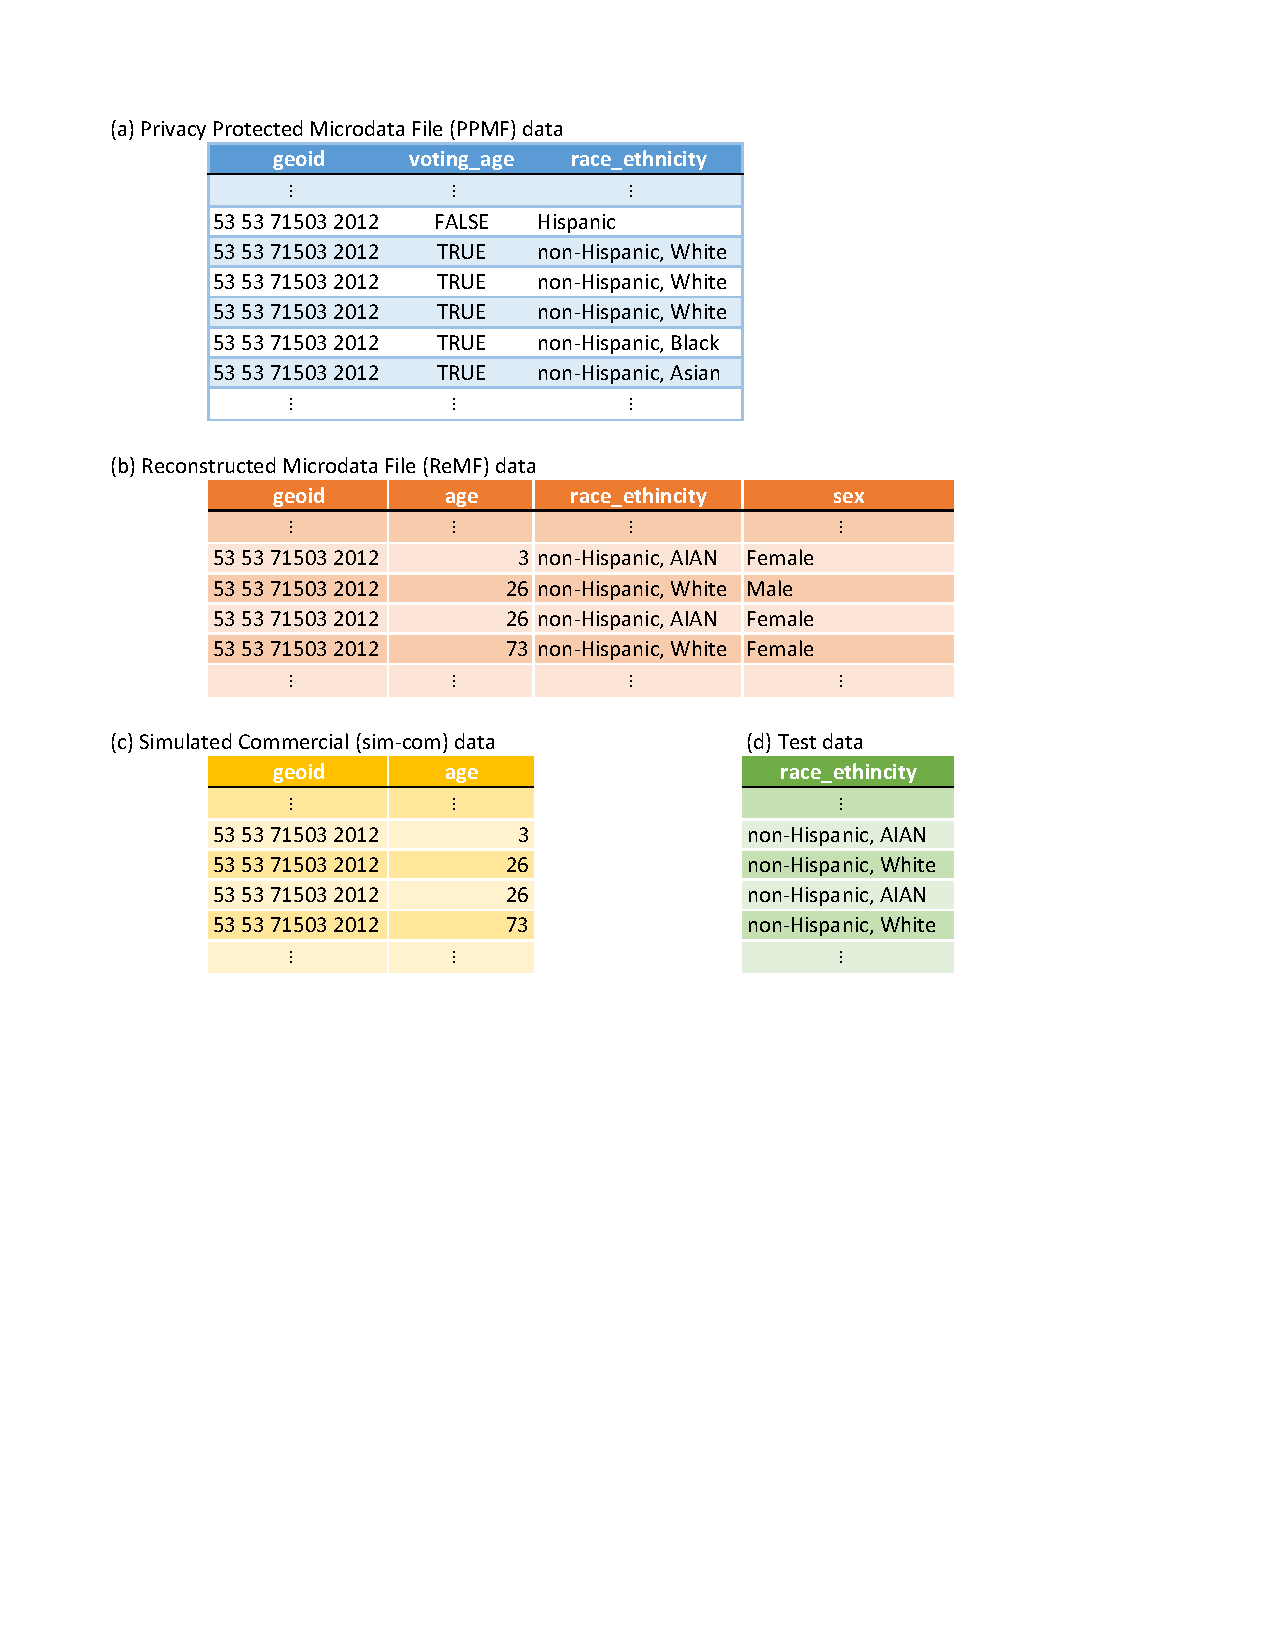
\includegraphics[width=\columnwidth]{tex/ppmf_reid_db_fig_cropped.pdf}}
\caption{Example rows from four databases used in a re-identification experiment: (a) Privacy-Protected Microdata File (PPMF) data, from Census Bureau or simulated; (b) Reconstructed Microdata File (ReMF) data, based on published tables from 2010 decennial census; (c) Simulated Commercial (sim-com) data, from \emph{some} columns of ReMF; (d) Test data, from other columns of ReMF (same rows as sim-com, different columns).}
\label{db}
\end{center}
\vskip -0.2in
\end{figure}

We then split our ReMF into a simulated commercial (sim-com) database and a test database (Figure~\ref{db}c and d), where the sim-com data contained the age, sex, and geographic detail (census block) for each individual in the ReMF who was not residing in group quarters, and the test data contained the race and ethnicity of each individual.

We merged records from the sim-com database to records from the PPMF, using exact record linkage on census block and voting-age status (i.e. $\mathbf{1}_{\mathrm{age} \geq 18}$) for individuals in the PPMF residing in households, and counted the number of individuals in the sim-com database who were linked to one or more individuals with a unique race/ethnicity value (putative links).  We also calculated the number and fraction of individuals for whom the unique linked race/ethnicity value matched the value in the test database (confirmed links).

For example, census block 2012 in census tract 71503 of King County, Washington contained 4 individuals in our sim-com data, only one of whom was not of voting age (a three-year-old female, first row of shown data in Figure~\ref{db}c).  A PPMF created with a large-enough value of $\epsilon$ would be highly likely to also contain a single non-voting-age individual in this block, and linking these records would risk disclosing the race and ethnicity reported by for this individual. A PPMF created with a sufficiently small value of $\epsilon$, on the other hand, would be likely to contain multiple people of non-voting age, with multiple race/ethnicity values, and therefore preclude re-identification of this child's race and ethnicity. In the $\epsilon=12.2$ PPMF, this block contained six individuals (Figure~\ref{db}a), only one of whom was of non-voting age, meaning re-identification yields a putative link for this child. However, the race/ethnicity data in the PPMF does not match that in the test data, so this link is \emph{not} confirmed, and the PPMF has succeeded in protecting the child's race and ethnicity attributes.

A limitation of our approach is that while the PPMF was constructed from the Census Edited File, we have derived our ReMF from published tables that were perturbed by the swapping algorithm that Census Bureau used for disclosure avoidance in the 2010 census, the details of which are secret \cite{mckenna2018disclosure}.   This means that a non-link or a non-confirmation of a link could be due to swapping, and could lead to an under- or over-estimation of the disclosure risk of the PPMF with $\epsilon=12.2$.  To further explore how differential privacy might protect PL-74 data, we also developed a simplistic proxy for PPMF data using a tunable $\epsilon$ and our ReMF data.  For each census block, we added laplace noise with parameter $\frac{1}{2\epsilon}$ to the histogram counts for strata of voting age times the 126 race/ethnicity combinations in census data, and then rounded the sums to the nearest non-negative integers.  We repeated our record linkage experiment with simulated PPMF data for a range of $\epsilon$ values ($\epsilon$-sim-PPMF).

To verify that our simulation was working as expected, we considered an $\epsilon=\infty$ sim-PPMF, for which we expected that all uniquely imputed race and ethnicity attributes should match the test data exactly, and we also considered an $\epsilon=0.01$ sim-PPMF, where we expected to find very few individuals with a uniquely imputed race or ethnicity, and even fewer where the imputed attribute would match the test data, i.e. at most a few correct matches, just by chance.

In addition to counting the total number of putative and confirmed re-identifications in our simulations, we also counted the putative and confirmed re-identifications among individuals of the non-majority race/ethnicity for their census tract.

\section{Results}

Our re-identification experiment produced the results we expected with the $\epsilon$-sim-PPMFs of very large and small $\epsilon$.  For $\epsilon=0.01$, we found zero putative re-identifications and therefore zero confirmed re-identifications from the sim-com data.  For $\epsilon=\infty$, we found 42.6 million putative links, of which all 42.6 million were confirmed (precision of 100\%).  This is re-identification of 13.6\% of the US population.

For the $\epsilon=12.2$ PPMF produced by TDA, we found 38.7 million putative re-identifications, of which 36.8 million were confirmed (precision of 95.1\%). This is putative re-identification of 12.4\% of the US population, and confirmed re-identification of 11.8\%.

When we restricted our attention to re-identification among people who were not of the majority race/ethnicity of their census tract, we found a substantial reduction in the re-identification.  For the $\epsilon$-sim-PPMF with $\epsilon=\infty$, we found 1.2 million putative links, and, since $\epsilon=\infty$ affords no privacy protection, all 1.2 million were confirmed for a precision of 100\%.  This is re-identification of XXX\% of the individuals who are not in the majority race/ethnicity group of their census tract, and YYY\% of the total US population.  Without privacy protection, non-majority re-identifications constitute ZZZ\% of all confirmed re-identifications.

For the $\epsilon=12.2$ PPMF produced by TDA, among people who were not of the majority race/ethnicity of their census tract, we found 1.5 million putative links (which we note is substantially \emph{more} than we found with the $\epsilon=\inf$ sim-PPMF).  However, we found only 0.6 million confirmed links, for a precision of XXX\%, substantially lower than the re-identification precision we found for the $\epsilon=12.2$ PPMF among the total population.  This is re-identification of XXX\% of the individuals who are not in the majority race/ethnicity group of their census tract, and YYY\% of the total US population.  For the $\epsilon=12.2$ PPMF, we found that non-majority re-identifications constitute ZZZ\% of all confirmed re-identifications.

[[perhaps a plot of the re-identification rate or precision among all and among non-majority groups, as a function of $\epsilon$?]]


\section{Discussion}

$\epsilon=\infty$ results demonstrat that without some disclosure avoidance system XXX\% of the US population would have had their race and ethnicity revealed in the 2010 PL-74 file.  Is this data really sensitive enough to deserve Title 13 protection?

$\epsilon=0.01$ results show that DP is quite capable of foiling this specific re-identification attack, and it turns out the even epsilon substantially larger than 0.01 precludes re-identification.

[[meaning of risk 12.2 among general population and non-majority population.]]

Balancing the trade-off between privacy and accuracy will always a policy decision, and in this case, it 
is a policy decision on a strict timeline.  We hope that the framework and results of our simulation study can be helpful to inform this debate and decision.


% In the unusual situation where you want a paper to appear in the
% references without citing it in the main text, use \nocite
%\nocite{langley00}

\bibliography{references}
\bibliographystyle{icml2021}




\end{document}

